\RequirePackage{luatex85}
\documentclass{standalone}
\usepackage{tikz}

% Color Definitions
%\definecolor{SourceColor}{RGB}{85,168,104}
\definecolor{SourceColor}{RGB}{255,255,255}
%\definecolor{TargetColor}{RGB}{221,132,82}
%\definecolor{TargetChangerColor}{RGB}{255,153,0}
\definecolor{TargetColor}{RGB}{255,255,255}
\definecolor{TargetChangerColor}{RGB}{255,255,255}
\definecolor{AbsorbingAreaColor}{RGB}{196,78,82}
\definecolor{ObstacleColor}{RGB}{179,179,179}
\definecolor{StairColor}{RGB}{129,114,178}
\definecolor{MeasurementAreaColor}{RGB}{255,0,0}
\definecolor{InformationAreaColor}{RGB}{0,255,0}
\definecolor{AerosolCloudColor}{RGB}{202,156,76}
\definecolor{AgentColor}{RGB}{76,114,202}
\definecolor{AgentIdColor}{RGB}{255,127,0}
\definecolor{ObstacleGreenColor}{RGB}{10,255,10}
\definecolor{ObstacleBlueColor}{RGB}{179, 236, 255}
\definecolor{ObstacleGreenColor}{RGB}{179, 255, 204}

\newcommand{\MeasurementAreaOpacity}{0.549020}
\newcommand{\AerosolCloudOpacity}{0.039216}

\usetikzlibrary{decorations.pathreplacing}

\begin{document}
\begin{tikzpicture}
\node[] at (0,0) {\includegraphics[width=12cm]{./unguided_364s.pdf} };

\node[] at (4.5,5) {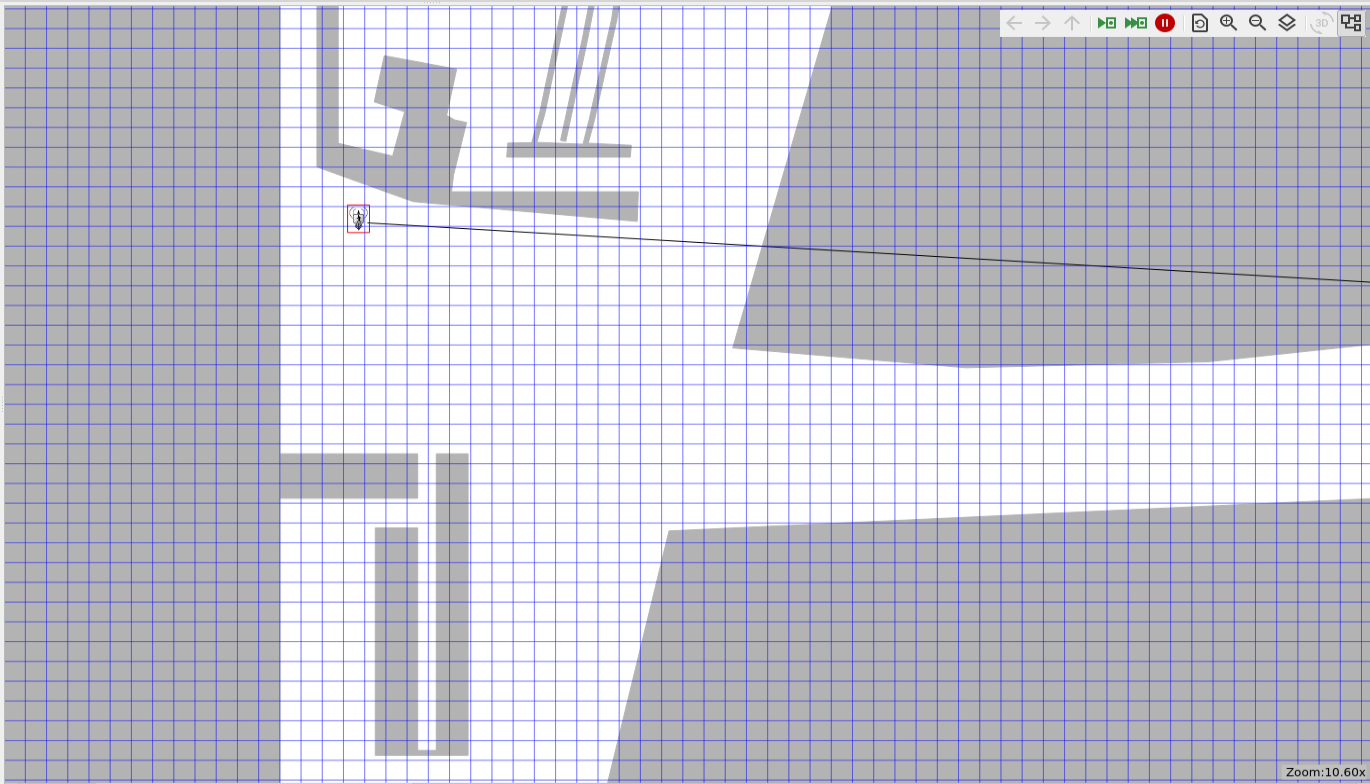
\includegraphics[width=6cm,clip,trim={5cm 0.0cm 18cm 1cm}]{./concept_2.png} };

\node[] at (-5.0,8.1) {Vadere GUI:};

\node[] at (-0.0,9) {OMNeT++ IDE: };
\node[] at (-1.4,-7.4) {50m};

\node[] (sourcea) at (-2.5,-1.7) {Source A};

\node[] (sourceb) at (0.3,-5.1) {Source B};

\node[] (targeta1new) at (0.4,-4.7) {Target A-1};



\draw [decorate,decoration={brace,amplitude=2pt,raise=4pt},yshift=0pt] (1.2,-4.5) -- (1.2,-5.3);



\node[] (targeta2) at (-2.1,-0.9) {Target A-2};

\node[]  at (2.5,-4.9) {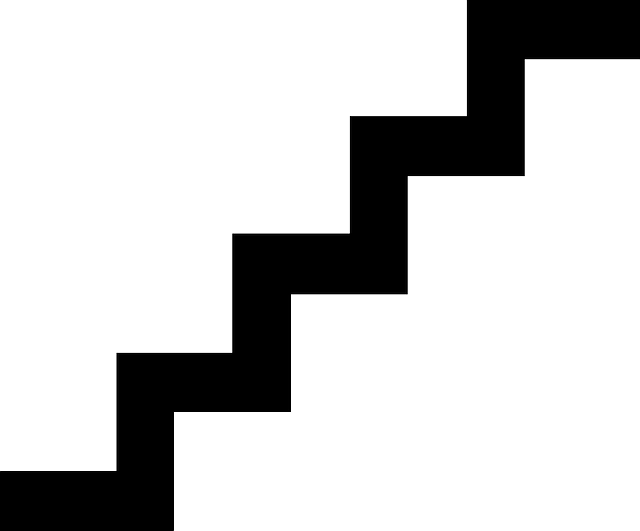
\includegraphics[width=0.6cm]{./stairs.png}};
\node[]  at (3.8,-4.9) {
\includegraphics[width=1cm]{./escalator2.png}};
\draw (1.8,-5.4) rectangle (4.4,-4.4);
\draw[->,line width=1mm, black!30!red]  (2.0,-5.2) -- (2.3,-4.9) ;
\draw[->,line width=1mm, black!30!blue]   (2.7,-4.5) -- (2.4,-4.8) ;

\draw[line width=0.5mm]   (3,-5) -- (3,-4.8) ;
\draw[line width=0.5mm]   (2.9,-4.9) -- (3.1,-4.9) ;


\draw[->]  (targeta1new) -- (-0.8,-4.7);
\draw[->]  (-0.5,-5.0) -- (-0.8,-4.8);




\node[] (targetb) at (-2.5,-3.4) {Target B};

\draw[] (-1.8,2.9) circle (0.4cm);
\draw[] (-0.8,4.3) circle (0.3cm);
\draw[] (-0.4,-0.6) circle (0.3cm);


\node[text width=5cm] (inter) at (-3.5,1.42) {Intermediate target: \\ target + target changer };

\draw[->] (inter) -- ++(1.4,1.2) ;

\draw[->]  (targeta2) -- ++(0.7,0.5);

\draw[->]  (targetb) -- (-1.2,-3.1);

\draw[->]  (sourcea) -- (-1.2,-2.1);

\node[text width=3cm] (relay) at (4.5,6.0) {Relay station \\ Base station};


\draw[->]  (relay) -- (3.6,7.0);


\node[text width=2cm] at (2.7,1) {Cell size:\\ 2m x 2m};

\node[] at (-4.3,-3.4) {
\includegraphics[width=1cm]{./bus.png} };
\draw[->,line width=1mm, black!30!red ] (-3.4,-3.4) -- (-4.3,-3.4) ;

\node[] at (-4.3,-1.7) {
\includegraphics[width=1cm]{./busR.png} };
\draw[->,line width=1mm, black!30!blue]  (-4.3,-1.7) -- (-3.4,-1.7) ;



\end{tikzpicture}
\end{document}
